\documentclass{beamer}

\mode<presentation> {
	\usetheme{Rochester}
	\setbeamertemplate{footline}[page number]
}

\usepackage{graphicx}
\usepackage{booktabs}

\title[NoSQL MongoDB vs. SQL ]{NoSQL MongoDB vs. SQL}

\author{}
\institute[UP]{
	Department of Computer Science, University of Pretoria
}
\date{\today}
\graphicspath{{pictures/}}

\begin{document}

\begin{frame}
	\titlepage
	\begin{center}
		\begin{tabular}{ c c c }
			Grobler, Arno & Harvey, Matthias & Lochner, Amy  \\
			\texttt{14011396} & \texttt{14027021} & \texttt{14038600} \\
			Madigoe, Pricilla & Maree, Armand & Obo, Diana \\
			\texttt{13049128} & \texttt{12017800} & \texttt{13134885} \\				
		\end{tabular}
	\end{center}
\end{frame}

\begin{frame}
	\frametitle{Overview}
	\tableofcontents
\end{frame}

	\section{Introduction}
		\begin{frame}
		\frametitle{Introduction}
	        \begin{itemize}
	            \item Misuse of database systems in industries 
				\item Studied research paper: Comparing NoSQL MongoDB to an SQL DB. Parker, Z. Poe, S. & Vrbsky, S.V. (2013)
				\item Purpose: To find where NoSQL and SQL databases can be used the most effectively.
			\end{itemize}
		\end{frame}
	
	\section{Database Problem Area}
		\begin{frame}
		\frametitle{Database Problem Area}
            \begin{itemize}
	            \item Most common database implementation is \textbf{relational model}.
				\item Not effective for \textbf{large} and \textbf{unstructured data}.
				\item Solution for large database could be to use \textbf{NoSQL}.
				\item However industry still needs \textbf{modest sized databases}.
				\item Can NoSQL be used then for modest sized databases?
			\end{itemize}
		\end{frame}
			
	\section{Advantages}
		\begin{frame}
		\frametitle{Advantages}
            \begin{itemize}
                MongoDB has better run-time performance for updates, deletes and selects over all where as SQL has better run-time performance for inserts overall.\hfill \break
                \blindtext
                    \begin{figure}[!htb]
                        \minipage{0.30\textwidth}
                            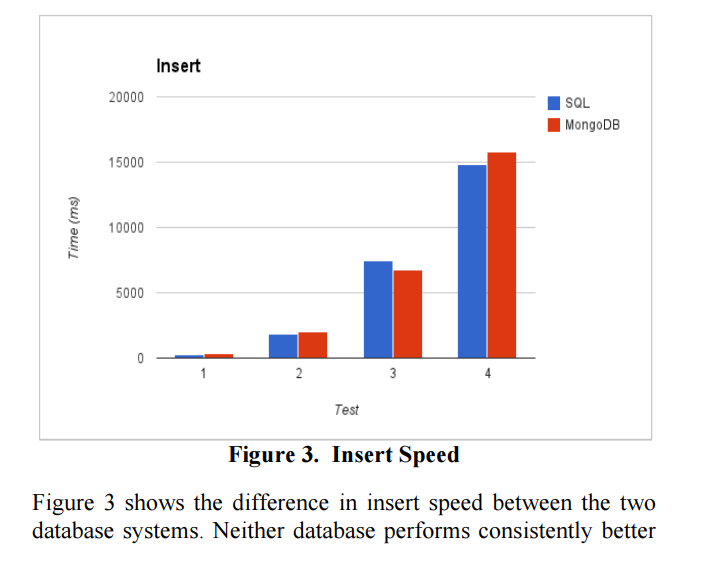
\includegraphics[width=\linewidth]{insert}
                        \endminipage\hfill
                        \minipage{0.30\textwidth}
                            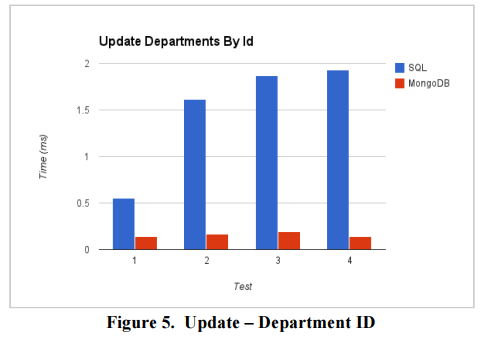
\includegraphics[width=\linewidth]{update}
                        \endminipage\hfill
                        \minipage{0.30\textwidth}
                            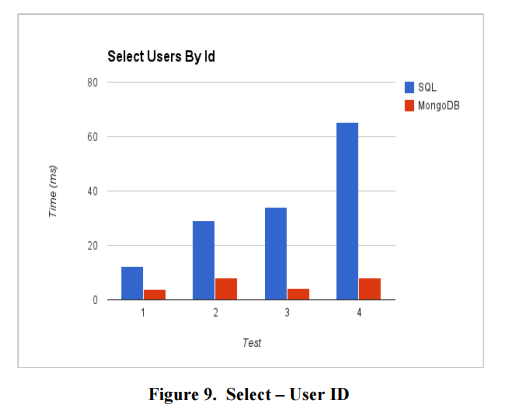
\includegraphics[width=\linewidth]{select}
                        \endminipage\hfill
                    \end{figure}
                \blindtext            
			\end{itemize}
		\end{frame}
		
	\section{Disadvantages}
		\begin{frame}
		\frametitle{Disadvantages}
            \begin{itemize}
	            \item MongoDB performs poorly for aggregate functions and querying based on non-key values
	            \item SQL DB requires additional joins in more complex schemas
	       \end{itemize}
		\end{frame}
		
	\section{Relevance to COS326 and the business industry}
		\begin{frame}
		\frametitle{Relevance to COS326 and the business industry}
		 \begin{itemize}
		     \item  Knowing the run-time performance on each databases helps one learn their various effective and efficient usage in real-world applications
		     \item Industry has evolved to require vast amounts of data
		     \item This data is usually unstructured since it is not always known in hindsight
		     \item Knowing about these databse systems could help one choose the best database for large volumes of data in terms of scalability and efficiency
		 \end{itemize}
		\end{frame}
		
	\section{Conclusion}
			\begin{frame}
			\frametitle{Conclusion}
                \begin{itemize}
                    \item The choice of NoSQL vs SQL is largely project dependent
                    \item Projects with dynamic schemas are generally better off using NoSQL because of its flexibility
                    \item The use of aggregate functions and querying based on non-key values is better suited to SQL
                    \item When high scalability is required, NoSQL is better suited because of its suitability to distributed computing
                \end{itemize}
			\end{frame}
\end{document} 
